\newif\iftwocol
\newif\ifplacefig
\newif\ifdraft
\newif\ifinclfig
\newif\ifieee

% For IEEE 
%\ieeetrue
%\twocoltrue
%\placefigtrue
%\inclfigtrue % false for word count (no figs)
%\draftfalse

% For Draft
\ieeetrue
\twocoltrue
\placefigtrue
\inclfigtrue
\drafttrue

% For ApJ preprint
%\ieeefalse
%\twocolfalse
%\placefigfalse
%\inclfigtrue
%\draftfalse

% For ArXiv
%\ieeefalse
%\twocoltrue
%\placefigtrue
%\inclfigtrue
%\draftfalse

%---------------------------------------------------------------------------------
% PREAMBLE
\iftwocol
	\ifieee
		\documentclass[journal]{IEEEtran}
	\else
		\documentclass[apj]{emulateapj}
	\fi
\else
	\ifieee
		\documentclass[peerreview]{IEEEtran}
	\else
		\documentclass[preprint]{aastex}
	\fi
\fi

\pdfoutput=1
\usepackage[normalem]{ulem}
\usepackage{color}
\usepackage{graphicx}
\usepackage{enumerate}
\ifdraft
	\ifieee
		\usepackage[numbers]{natbib}
		\bibliographystyle{ieeetr}
	\else
		\usepackage{natbib}
		\citestyle{apj}
		\bibliographystyle{apj}
		\bibpunct[,]{(}{)}{;}{a}{}{,}
	\fi
\else
	\ifieee
		\usepackage[numbers]{natbib}
		\bibliographystyle{ieeetr}
	\fi
\fi

\usepackage[bookmarks=false]{hyperref}

\ifieee
\usepackage{etoolbox}
\makeatletter
\patchcmd{\@makecaption}
  {\scshape}
  {}
  {}
  {}
\makeatletter
\patchcmd{\@makecaption}
  {\\}
  {.\ }
  {}
  {}
\def\tablename{Table}
\makeatother
\else
%\makeatletter
\fi

%---------------------------------------------------------------------------------
% CONTROL THINGS
\newcommand{\todo}[1]{{\color{red}{#1}}}
\newcommand{\addref}{{\color{red}(ref. needed)}}
\newcommand{\Msol}{\,M$_{\odot}$}
\newcommand{\TB}{\,Tbytes}
\newcommand{\cis}{{\tt cis\_interface}{}}

%---------------------------------------------------------------------------------
% MANUSCRIPT INFO
\begin{document}

\ifieee
\else
	\shorttitle{{\cis}}
\fi

\title{{\cis}: A Python Package for Integrating Computational Models Across Languages and Scales}

\ifieee
	\author{Meagan~Lang%
	\thanks{The authors are with the National Center for Supercomputing Application, University of Illinois, Urbana-Champaign, IL 61801 USA (e-mail: langmm@illinois.edu)}}
\else
	\author{Meagan~Lang\altaffilmark{1}}

	\altaffiltext{1}{National Center for Supercomputing Application, University of Illinois, Urbana-Champaign, IL email: {\tt langmm@illinois.edu}}
\fi


\ifieee
	\maketitle
\fi

%---------------------------------------------------------------------------------
% ABSTRACT (145 words)
\begin{abstract}
Thousands of computational models have been created within the plant biology community in the past two decades that have the potential to be combined into complex integration networks capable of capturing more complex biological processes than possible with isolated models. However, the technological barriers introduced by differences in language and data formats has slowed this progress. We present \href{https://github.com/cropsinsilico/cis_interface}{\cis}, a Python package for running integration networks with connections between models across languages and scales. {\cis} coordinates parallel execution of models in Python, C, C++, and Matlab on Linux, Mac OS X, and Windows operating systems, and handles communication in a number of data formats common to computational plant modeling. {\cis} is designed to be user-friendly, with visual tools developed in parallel for composing the integration networks. 
\end{abstract}

\ifieee
	\begin{IEEEkeywords}
		Plant modeling, Modeling, Communication
	\end{IEEEkeywords}
	\IEEEpeerreviewmaketitle
\else
	\maketitle
\fi

%---------------------------------------------------------------------------------
%---------------------------------------------------------------------------------
% INTRO (183 words)
\section{Introduction}\label{S:intro}
%
%\IEEEPARstart{C}{omputational} 
Computational plant biologists have produced a wealth of computational models to describe the biological processes governing plant growth and development, covering scales from atomic to global. Although usually developed independently to address questions specific to an organ, species, or growth process, computational plant models can also have applications beyond their original scope. Many biological processes are the same across different species of plants, allowing models developed for one species to be adapted for another by modifying input parameters. In addition, computational models for different scales, organs, or processes can also be combined, or integrated, to probe more complex biological mechanisms. By integrating a metabolic flux model with a genetic regulatory model for carbon uptake, 
%
\ifieee
	\citep{integration_prep} 
\else
	\citet{integration_prep} 
\fi
%
was able to identify gene candidates for regulating photosynthesis under elevated CO$_{2}$. With advances in compute power, it should be possible to link biologically related models to create complex integration networks capable of capturing the response of entire plants, fields, or regions. However, independently developed computational models often have compatibility issues resulting from differences in programming language or data format that make such collaborations difficult. 

We present an Open Source Python package, {\cis}, for creating and running integration networks by connecting existing computational models written in Python, Matlab, C and C++. Although developed for the purpose of integrating plant biology models, {\cis} can be applied to any situation requiring coordination between models in the supported languages. \S\ref{S:background} provides background information on existing efforts for cross-language model integration, \S\ref{S:methods} describes the methods used by the {\cis} package to integrate models, \S\ref{S:results} presents several tests demonstrating the performance of message passing between integrated models, and \S\ref{S:discuss} summarizes the features of the {\cis} package, describes a few use cases, and outlines areas for future development.

%---------------------------------------------------------------------------------
%---------------------------------------------------------------------------------
% BACKGROUND
\section{Background}\label{S:background}
%
Computational plant models are usually written with a very specific research question in mind. The resulting programs are highly tuned for one purpose and written specifically for scientists within an isolated group of collaborators. Scientists will generally write programs in the language they are most familiar with and, given that there is no consensus on one programming language as ideal for all scientific applications, the language of computational models will often vary between research groups, if not between members of the groups themselves. The same can be said of data formats which can be highly tailored to the target question and may or may not include metadata like the data types, field names, or units. To integrate two biological models, the following questions must be addressed:
%
\begin{enumerate}
	\item Orchestration: How will models be executed?
	\item Communication: How will information be passed from one model to the next across languages?
	\item Translation: How will data output by one model be translated into a format understood by the next model?
	%\item Computational Efficiency: Will the integration make good use of computational resources?
	%\item Human Efficiency: How much hands-on work will the integration take and can products be reused in the future?
\end{enumerate}

These three questions can be addressed through manual integration on the command line or using scripting (e.g. running model A, converting output from A into input expected by model B, running model B). However, manual integration is 1) computational inefficient when many iterations are necessary, such as during parameter searches or steady state convergence tests, 2) unique to every integration, requiring the production of new scripts, and 3) complex when more than $>3$ models are being integrated. Within both computational biology and the larger scientific computing community, groups have developed around different solutions to the problem of connecting models.

%---------------------------------------------------------------------------------
% DOMAIN SPECIFIC LANGUAGE
\subsection{Domain Specific Language (DSL)}\label{SS:dsl}
%
One solution is to agree upon a language. The questions of orchestration, communication, and translation become trivial when models are all written in the same language. Beyond selecting a single programming language, many communities have  developed dedicated domain specific languages (DSLs) for model representation. For example, the Systems Biology Markup Language \citep[SBML][]{Hucka2003} is an XML-based format for representing models of biological processes. Scientists can compose their models using SBML markup and then run their model using software designed to parse SBML files. Other DSLs for biological models include LPy \citep{Boudon2012}, CellML \citep{Cuellar2003}, and BioPAX \citep{Demir2010}. Dedicated model DSLs improve the reusability of models written in the DSL and have the advantage of often implicitly handling data transformation. However, they do nothing for existing models that are not in the DSL or cannot be expressed within the constraints of the DSL. In addition, learning a new DSL, in addition to a programming language, can be daunting for new researchers.

%---------------------------------------------------------------------------------
% FRAMEWORKS
\subsection{Workflow/Data Flow/Framework}\label{SS:framework}
%
Another approach is a workflow/data flow/framework tool for models that are written in the same programming language or can be wrapped. For example, there are many generic tools in Python for coordinating the execution of tasks in parallel or serial \citep[e.g.][]{babuji18, celery, luigi}. While these tools are powerful for organizing complex work flows, it is the user's onus to make sure that the components they connect are compatible and handle any data transformation that might be necessary (e.g. unit conversion or field selection).

There are also domain specific frameworks for connecting biological models. For example, OpenAlea \citep{Pradal2015} allows users to compose networks from different components including plant models, analysis tools, and visualization tools. Domain specific frameworks are more intuitive and ultimately more flexible than DSLs in the types of operations they allow models to perform since they have access to the full power of a programming language. However, they are stricter in several respects: 1) the model must be written in (or exposable to), the language of the framework and 2) the model must be written in a way that is aware of the framework and/or the format of models with which it will interact. Like DSLs, frameworks also provided limited support for models written without them in mind. 

{\cis} interface is an example of a framework that overcomes these issues by exposing light-weight interfaces in the language of the model (See \S\ref{SSS:interface}) that permit messages to be passed between the model processes as they run in parallel (See \S\ref{SS:communication}). As a result, models writers only need knowledge of the language in which their model is written.

%---------------------------------------------------------------------------------
% MESSAGE PASSING TOOLS
%\subsection{Message Passing Tools}\label{SS:messages}
%
%There are many existing software solutions for passing messages between processes. Implementations of the Message Passing Interface (MPI) standard, such as MPICH \citep{Gropp1996} and OpenMPI \citep{Gabriel2004}, allow communication between instances of a program launched on parallel processes with distributed memory. MPI implementations are robust, fast, and scale well, however, they are optimized for processing high volumes of structured data on supercomputers and are not as well suited to the case of dynamic integration networks composed of diverse processes operating on different timescales.

%---------------------------------------------------------------------------------
%---------------------------------------------------------------------------------
% METHODS
\section{Methods}\label{S:methods}

{\cis} was designed to address the questions from \S\ref{S:background} while being:

\begin{itemize}
	\item Easy to use. Require as little modification to the model source code as possible and only in the language of the model itself.
	\item Efficient. Allow models to run in parallel with asynchronous communication that dosn't block when a message is sent.
	\item Flexible. Provide the same interface to the user, regardless of the communication mechanism being used or the platform the model is being executed on.
\end{itemize}

{\cis} currently support models written in Python, Matlab, C, and C++ with 
additional Domain Specific Language (DSL) support for LPy models \citep{Boudon2012}. 

%---------------------------------------------------------------------------------
% ORCHESTRATION
\subsection{Orchestration}\label{SS:orchestration}
%
{\cis} is executed via a command line interface (CLI), {\tt cisrun} with YAML specification files (\S\ref{SSS:yaml}) as input. Based on the information contained in the YAML specification files, {\cis} establishes a network of asynchronous communication channels (\S\ref{SS:communication}), and launches the models on new processes (\S\ref{SS:model_driver}).
%At execution, {\cis} launches models on new processes based on information contained in a YAML specification file (See \S\ref{SSS:yaml} below) and establishes 

%---------------------------------------------------------------------------------
% YAML
\subsubsection{YAML Specification}\label{SSS:yaml}
%
Users specify information about models and integration networks via declarative 
YAML files \citep{Ben-Kiki2009}. The YAML file format was selected because it is human readable 
and there are many existing tools for parsing YAML formats in different programming 
languages. The declarative format allows user to specify exactly what they 
want to do, without describing how it should be done. While the information 
about models and integration networks can be contained in a single YAML 
file, the information can naturally be split between two or more files, one (or more) containing 
information about the model(s) and one containing the connections comprising the 
integration network. This separation is advantageous because the model YAML 
can be re-used, unchanged, in conjunction with other integration networks. 

Model YAMLs include information about the location of the 
model source code, the language the model is written in, how the model should 
be run, and any input or output variables including their data type and units. 
Integration networks are specified via YAML files declaring the connections 
between models. Connections are declared by pairing an output variable from 
one model with the input variable of another model. The {\cis} 
CLI sets up the necessary communication mechanisms to 
then direct data from one model to the next in the specified pattern. Models 
can have as many input and/or output variables as is desired.
Connections between models are specified by references to the 
input/output variables associated with each model. This format allows users the 
flexibility to create complex integration networks. 

%---------------------------------------------------------------------------------
% LANGUAGE SUPPORT
%\subsubsection{Language Support}\label{SSS:language}
%
%{\cis} currently support models written in Python, Matlab, C, and C++ with 
%additional Domain Specific Language (DSL) support for LPy models \citep{Boudon2012}. 
%Support for model languages is achieved through a language specific driver and API.

%---------------------------------------------------------------------------------
% MODEL DRIVERS
\subsubsection{Model Drivers}\label{SS:model_driver}
%
Model drivers handle model execution, monitoring, and compilation if necessary. 
While every model is executed on a new process, how the model is handled depends 
on the language it is written in. Models written in 
interpreted languages (Python and Matlab) are executed on the command line 
with the interpreter. In the case of Matlab, where there is significant overhead 
associated with starting the Matlab interpreter (See \S\ref{SS:results_language}), a Matlab shared engine is used 
to execute the model. To speed up the execution, the shared engine can be started 
in advance and then reused.

For the compiled languages (C and C++) there are a few options. The user can 
compile the model themselves, provided they link against the appropriate 
{\cis} header library. Alternatively, users can provide the location of 
the model source code and let {\cis} handle the compilation, including 
linking against the appropriate {\cis} header library. {\cis} 
also has support for compiling models using Make \citep{Stallman2004} and 
CMake \citep{Martin2006} for 
models that already have a Makefile or CMakeLists.txt. To use these drivers, 
lines are added to the recipe in order to allow linking against {\cis}.

Once model are running, each model driver uses a thread to monitor the progress of the model and report back model output (e.g. log messages printed to stdout) and any status changes to the master process. If a model issues any errors, the master process will shut down any model processes that are still running. If a model completes without any errors, the master process will cleanup any input/output channels that are no longer required. The master process will only complete once an error is encountered or all model processes have completed.


%---------------------------------------------------------------------------------
% COMMUNICATION
\subsection{Communication}\label{SS:communication}
%
Communication within {\cis} was designed to be flexible in terms of the 
languages, platforms, and data types. To accomplish this, {\cis} leverages 
several tools different tools for communication which are applied as needed. The 
particular mechanism used by {\cis} for communication is hidden from the 
user, who will always use the same interface in the language of their model 
(See \S\ref{SSS:interface}). 

%---------------------------------------------------------------------------------
% ASYNCHRONOUS MESSAGE MASSING
\subsubsection{Asynchronous Message Passing}\label{SSS:async}
%
Regardless of the specific communication mechanism, the same asynchronous
communication strategy is used. Models do not block on sending messages to 
output channels; the model is free to continue working on its task while 
a separate thread waits for the message to be routed and received. Similarly, 
a thread continuously pings input channels, moving received messages into a 
buffer queue so that they are ready and waiting for the receiving model 
when it asks for input. As a result, models in complex integration networks 
can work in parallel, improving the overall efficiency with which computational 
resources are used. Figure \ref{fig:async} describes the general flow of messages.
%
\ifinclfig
 	\begin{figure}[htbp]
	\begin{center}
	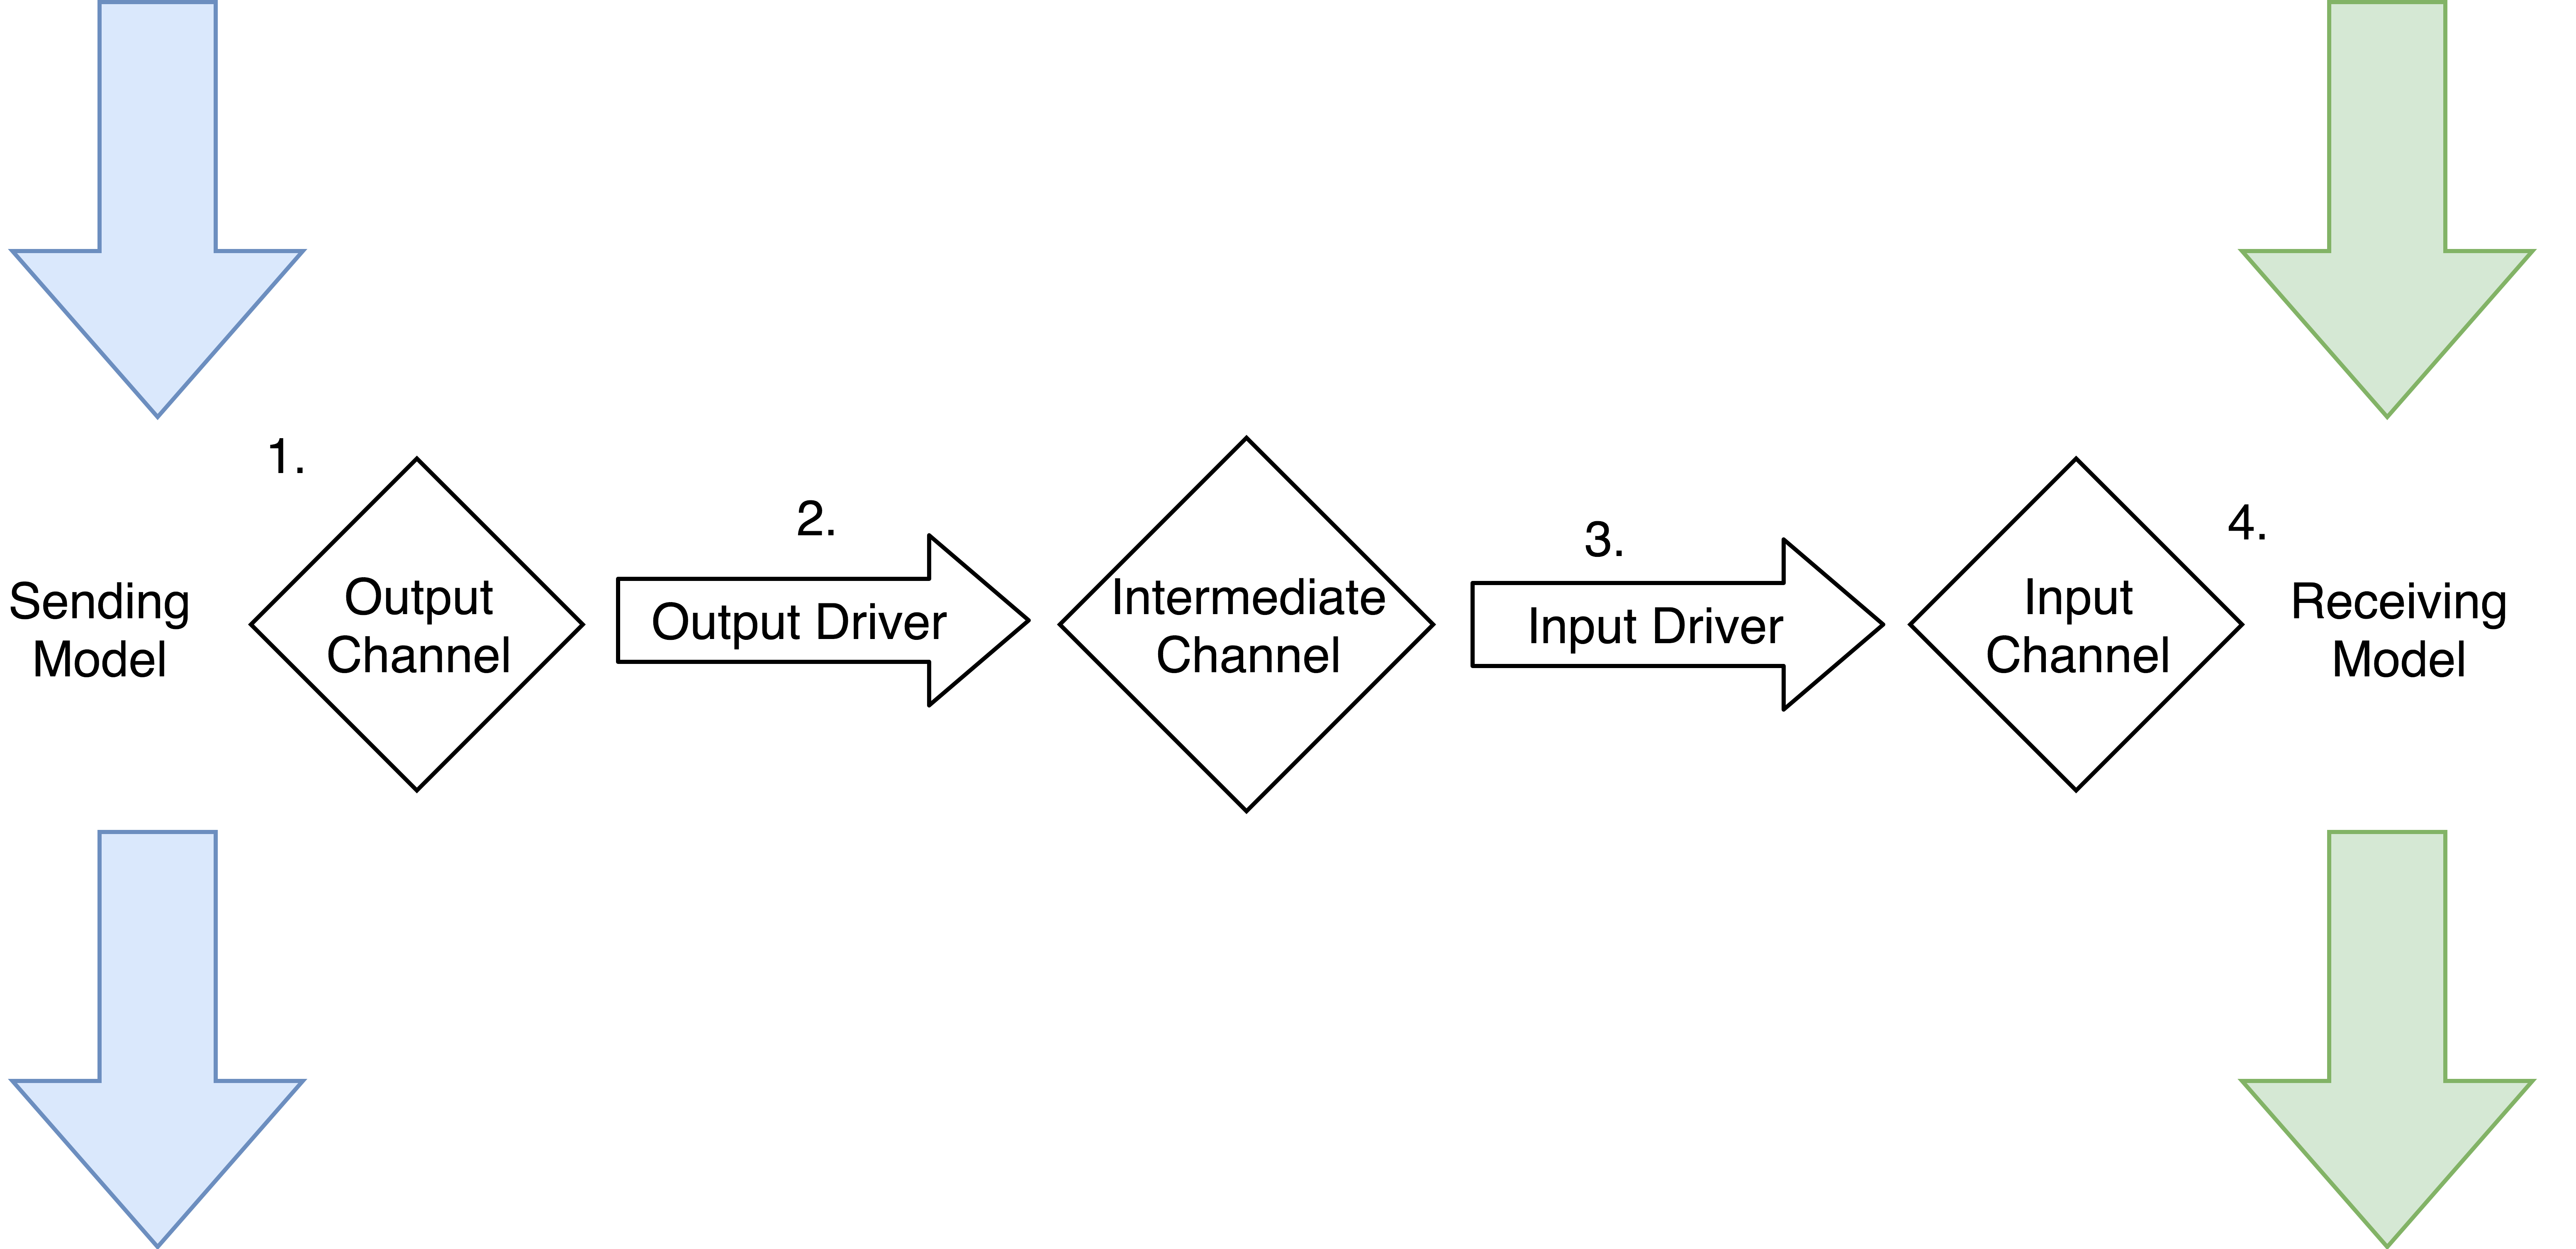
\includegraphics[width=\columnwidth,keepaspectratio]{./images/io_drivers.png}
	\caption{Diagram of how messages are passed asynchronously using input/output drivers and an intermediate channel.}
	\label{fig:async}
	\end{center}
	\end{figure}
\fi
%
\begin{enumerate}
	\item A model sends a message in the form of a native data object via a language 
specific API to one of the output channels declared in the model YAML. The output channel interface encodes the message and sends it.
	\item An output connection driver (written in Python) runs in a separate thread, listening to the model output channel. When the model sends a message, the output connection driver checks that the message is in the expected format and then forwards it to an intermediate channel. The intermediate channel may seem unnecessary, but it is used as a buffer for future support on distributed architectures (e.g. if one model is running on a remote machine). In these cases, the intermediate channel will connect to a RabbitMQ broker using security credentials.
	\item An input connection driver (also written in Python) runs in a separate thread, listening to the intermediate channel. When a message is received, it is then forwarded to the input channel of the receiving model as specified in the integration network YAML.
	\item The receiving model receives the message in the form of an analogous native data object.
\end{enumerate}

In addition to communication between two models, users can also specify that a 
model should receive/send input/output from/to a file. This is specified in 
the integration network YAML and does not impact the way the model will 
receive/send messages. In this way, users can test their model integration in 
isolation with input/output form/to files rather than another model.

%---------------------------------------------------------------------------------
% SYSTEM V IPC
\subsubsection{System V IPC Queues}\label{SSS:ipc}
%
The first communication mechanism used by {\cis} was System V interprocess 
communication (IPC) message queues \citep{Rusling1999} on Posix (Linux and Mac OS X) systems. 
IPC message queues allow messages to be passed between models running on separate 
processes on the same machine. While IPC message queues are light weight, fast 
(See \S\ref{SS:results_commtype}), and are part of Posix operating systems, they do not work in all 
situations. Sys V IPC queues are not natively supported by Windows operating systems 
and do not allow communication between remote processes. In addition, IPC queues also 
have relatively low default message size limits on Mac OS X systems (2048 bytes). Once 
the queue is full or if the message is larger than the limit, any process attempting to send an additional message will block until a 
sufficient number of messages has been removed from the queue to accommodate the new message. 
For messages larger than the limit, the sending process will block indefinitely. 
This can be handled by splitting large messages into multiple smaller messages 
(See \S\ref{SSS:large}), however, the time required to send a message increases with the number of 
message it must be broken into (See \S\ref{SS:results_commtype}). These limits make sending large messages 
relatively inefficient when compared with other communications mechanisms. 
As a result, Sys V IPC queues are used by 
{\cis} as a fallback on Posix systems if the necessary ZeroMQ libraries have 
not been installed.

%---------------------------------------------------------------------------------
% ZEROMQ
\subsubsection{ZeroMQ}\label{SSS:zmq}
%
The preferred communication mechanism used by {\cis} are ZeroMQ sockets 
\citep{Akgul2013}. ZeroMQ 
provides broker-less communication via a number of protocols and patterns with 
bindings in a wide variety of languages that can be installed on Posix and Windows 
operating systems. ZeroMQ was adopted by {\cis} in order to allow support 
on Windows and for future target languages (See \S\ref{SS:future}) that could not be 
accomplished using System V IPC queues. In addition, while ZeroMQ allows 
interprocess communication via IPC queues like System V IPC queues, ZeroMQ also 
supports protocols for distributed communication via an Internet Protocol (IP) 
network. While {\cis} does not currently support using these protocols 
for distributed integration networks, this is part of the plans for future improvement.

%---------------------------------------------------------------------------------
% RABBITMQ
\subsubsection{RabbitMQ}\label{SSS:rmq}
%
While ZeroMQ provides broker-less communication means, {\cis} includes support 
for brokered communication via RabbitMQ \citep{RMQ}. {\cis} does not currently use 
RabbitMQ for communication unless explicitly specified by the user in their 
integration network YAML. RabbitMQ support was originally added to {\cis} 
as a supplement to System V IPC queues in the case of future support for distributed 
integration networks. In future development, RabbitMQ brokered communication will be 
used for establishing integration networks with remote models run a services 
(See \S\ref{SS:future}).

%---------------------------------------------------------------------------------
% SENDING/RECEIVING LARGE MESSAGES
\subsubsection{Sending/Receiving Large Messages}\label{SSS:large}
%
All of the communication tools leveraged by {\cis} have intrinsic limits 
on the allowed size for a single message. Some of these limits can be quite large 
($2^{20}$ for ZeroMQ and RabbitMQ), while others are very limiting 
(2048 on Mac OS X for Sys V IPC queues). Although messages consisting of a few scalars are unlikely to 
exceed these limits, biological inputs and outputs are often much more complex. 
For example, structural data represented as a 3D mesh can easily exceed these 
limits. To handle messages that are larger than the limit of the communication 
mechanism being used, {\cis} splits the message up into multiple smaller 
messages. In addition, for large messages, {\cis} creates new, temporary 
communication channels that are used exclusively for a single message and 
then destroyed. The address associated with the temporary channel is sent in 
header information as a message on the main channel along with information about 
the message that will be sent through the temporary channel like size and data type. 
Temporary channels are used for large messages to prevent mistakenly combining 
the pieces from two different large messages that were received at the same time 
such as in the case that a model is receiving input from two different models 
working in parallel.

%---------------------------------------------------------------------------------
% INTERFACE
\subsubsection{Interface}\label{SSS:interface}
%
{\cis} provides interface functions/classes for communication that are 
written in each of the supported languages. Language specific interfaces 
allow users to program in the 
language(s) with which they are already familiar. The Python interface provides 
communication classes for sending and receiving messages. The Matlab 
interface provides a simple wrapper class for the Python class, that exposes 
the appropriate methods and handles conversion between Python and Matlab 
data types. The C interface provides structures and functions for accessing 
communication channels and sending/receiving messages. The C++ interface 
provides classes that wrap the C structures with functions called as methods.

In addition to basic input and output, each interface also provides access 
to more complex data types and communication patterns.


%---------------------------------------------------------------------------------
% SERIALIZATION
%
\subsection{Transformation}\label{SS:transformation}
%
%\subsubsection{Data Formats}\label{SSS:dataformats}
%
Messages are passed as raw bytes. In order to understand the messages begin passed, parallel processes that communicate must agree upon the format used to do so. Without community standards, different models will often use very different data formats for their input and output. Differences between data formats can include, but are not limited to, type, precision, fields, or units. While some data formats are self-descriptive and include these types of information as meta data, this is not true of all data formats. To combat this, {\cis} requires models to explicitly specify the format of input and output expected by a model in the model YAML. {\cis} can then handle a number of conversion between models without prompting as well as serialization/deserialization to the correct type in each of the supported languages. Data formats currently supported by {\cis} include:
%
\begin{itemize}
	\item Scalars (e.g. integers, floats)
	\item Arrays
	\item Tabular (e.g. CSV or tab-delimited)
	\item Pandas data frames
	\item PLY
	\item OBJ
\end{itemize}

%\subsubsection{Units}\label{SSS:units}
%
In addition, {\cis} offers the option to specify units for scalars, arrays, tabular data, and pandas data frames. Units are tracked using the {\tt unyt} package \citep{Goldbaum2018}. If two models use different units (and both are specified), {\cis} will automatically perform the necessary conversions before passing data from one model to the next.

%---------------------------------------------------------------------------------
%---------------------------------------------------------------------------------
% RESULTS
\section{Results}\label{S:results}
%
In order to evaluate {\cis}, performance tests were run on machines with Linux, Mac OS X, and Windows operating systems for different communication mechanisms, Python versions, and language combinations. During each run, $N_{msg}$ messages of size $S_{msg}$ were sent from the source model (in one language) to the destination model (in another language) which then output the messages to file for verification. Performance tests were run using the perf package \citep{Stinner2018}. Each run was repeated 10 times to rule out fluctuations due to external loads on the test machines.

% COMMTYPE
\subsection{Communication Mechanism}\label{SS:results_commtype}
%
Figure \ref{fig:commtype} compares the execution times for the different communication mechanisms discussed in \S\ref{SS:communication} for sending different numbers/sizes of messages from one Python model to another Python model. The tests were run on a Dell tower with Dual Intel(R) Xeon(R) CPU E5-2650 v3 @ 2.30GHz processors running Ubuntu 14.04. The left panel of Figure \ref{fig:commtype} shows the total time required to run both models and send a varying number of 1000 bytes messages from one model to the other. The right panel of Figure \ref{fig:commtype} shows the total time required to run the models and send 5 messages of varying lengths from one to the other. 
%
\ifinclfig
 	\begin{figure}[htbp]
	\begin{center}
	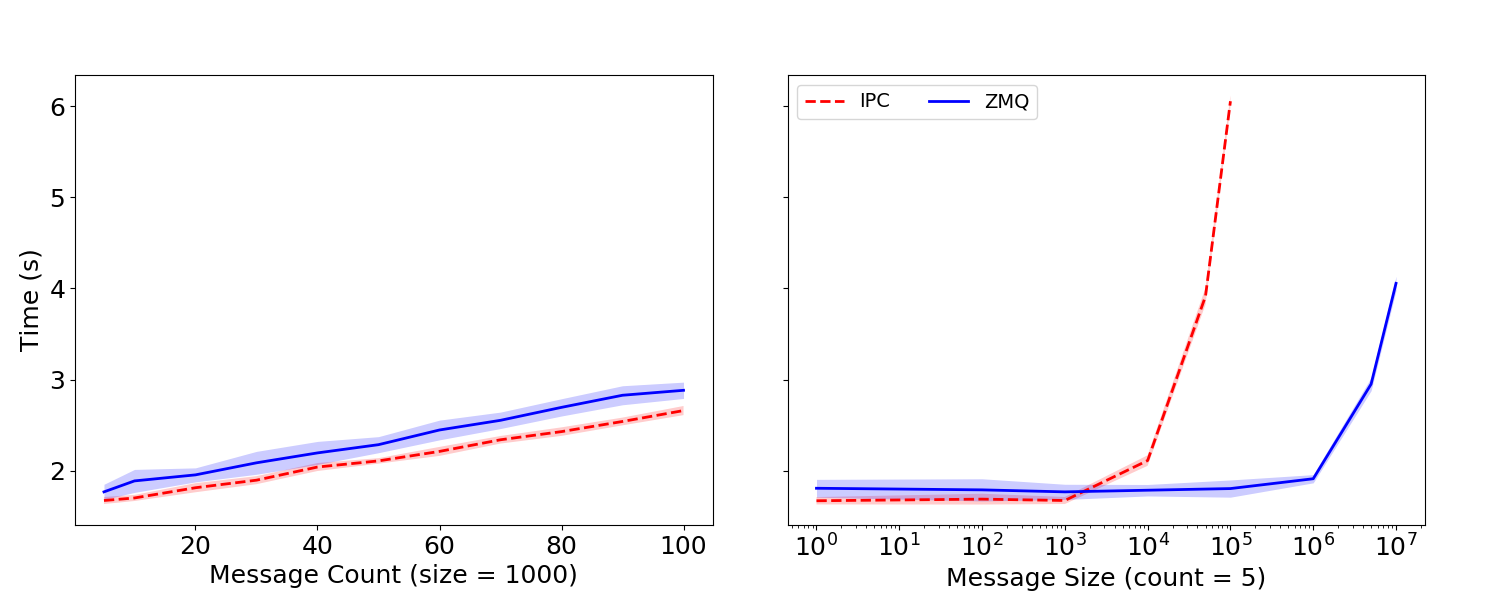
\includegraphics[width=\columnwidth,keepaspectratio]{./images/scaling_commtype.png}
	\caption{Comparison of communication time scaling across communication methods on Linux. Lines show the average run time for each test with the standard deviation shown in the shaded region. Left: Scaling of execution time with number of 1000 byte messages sent. Right: Scaling of execution time with the size of the 5 messages sent.}
	\label{fig:commtype}
	\end{center}
	\end{figure}
\fi
%

Table \ref{tab:commtype} shows how the two communication mechanisms compare as determined by performing a linear fit to the scaling of execution time with message count from Figure \ref{fig:commtype}. Time per message (slope of Figure \ref{fig:commtype}) is the average amount of time required to send a single message containing 1000 bytes and constrains how quickly messages can be passed between the models. Overhead (intercept of Figure \ref{fig:commtype}) is the amount of execution time that would be required if no messages were passed between the models and includes the time required to set up communication mechanisms, start the model drivers, and clean up the integration network.
%
\begin{table}[htbp]
%\caption{The time required per message and overhead for startup/teardown of integration for different communication mechanisms as determined by a linear fit to the scaling of execution time with message count. }
\begin{center}
\begin{tabular}{|c|c|c|}
\hline
Mechanism	& Time per Message (s) 	& Overhead (s) 	\\\hline
IPC			& 0.010				& 1.60			\\
ZMQ 		& 0.012				& 1.73			\\\hline
\end{tabular}
\end{center}
\caption{Effect of communication mechanism on performance.}
\label{tab:commtype}
\end{table}%
%
Although Sys V IPC queues are slightly faster than ZeroMQ TCP sockets in both time per message and overhead for messages smaller than the limit, IPC queues have a much smaller maximum size limit for messages. As discussed in \S\ref{SSS:large}, messages larger than this limit (2048 bytes) must be broken up into multiple messages, compounding the time required to send these messages and making IPC queues a poor choice for sending data over $\sim10^5$ bytes. This limit is much larger for ZeroMQ sockets ($\sim10^6$ bytes). However, for messages less than the limit, both ZMQ and IPC communication has no measurable dependence on message size.

% LANGUAGE
\subsection{Language}\label{SS:results_language}
%
Figure \ref{fig:language} compares the execution times for integrations with communications between models in different combinations of languages and Table \ref{tab:language} reports the time per message and overhead. The runs for Figure \ref{fig:language} and Table \ref{tab:language} were run on the Linux machine from above while those for Figure \ref{fig:language_matlab} and Table \ref{tab:language_matlab} were run on a 2015 MacBook Pro with a 2.9 GHz Intel Core i5 processor running macOS High Sierra 10.13.4 that had Matlab R2017a installed. In both cases, ZeroMQ communication was used with Python 2.7.
%
\ifinclfig
 	\begin{figure}[htbp]
	\begin{center}
	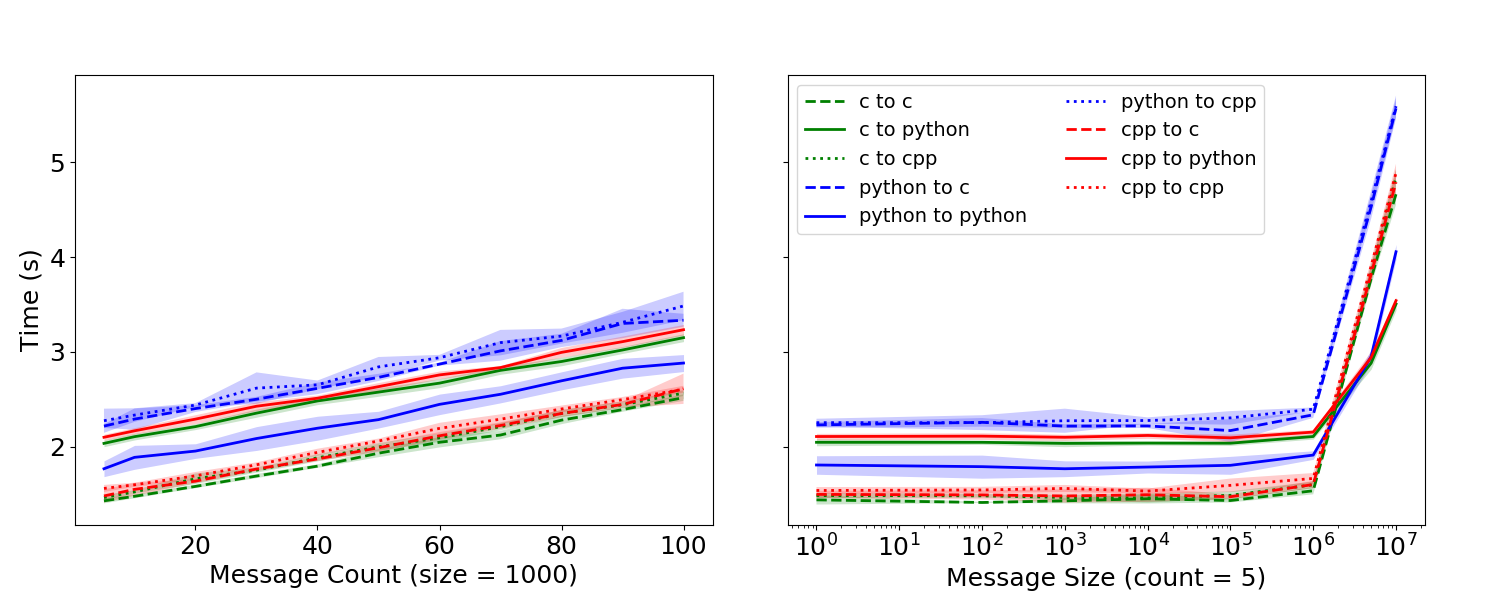
\includegraphics[width=\columnwidth,keepaspectratio]{./images/scaling_language.png}
	\caption{Comparison of communication time scaling between languages on Linux without Matlab. The same fiducial message size (1000 bytes) and count (5) was used as in Figure \ref{fig:commtype}.}
	\label{fig:language}
	\end{center}
	\end{figure}
\fi
%
\begin{table}[htbp]
\begin{center}
\begin{tabular}{|c|c|c|c|}
\hline
Source 	& Destination 	& Time per Message (s) 	& Overhead (s) 	\\\hline
C 				& C					& 0.011				& 1.36			\\
C 				& C++				& 0.012				& 1.42			\\
C 				& Python				& 0.012				& 1.99			\\
\hline%
C++ 				& C					& 0.012				& 1.42			\\
C++ 				& C++				& 0.011				& 1.49			\\
C++ 				& Python				& 0.012				& 2.05			\\
\hline%
Python			& C					& 0.012				& 2.15			\\
Python			& C++				& 0.012				& 2.21			\\
Python			& Python				& 0.012				& 1.73			\\
\hline
\end{tabular}
\end{center}
\caption{Effect of model language on performance (Linux).}
\label{tab:language}
\end{table}%
%
\ifinclfig
 	\begin{figure}[htbp]
	\begin{center}
	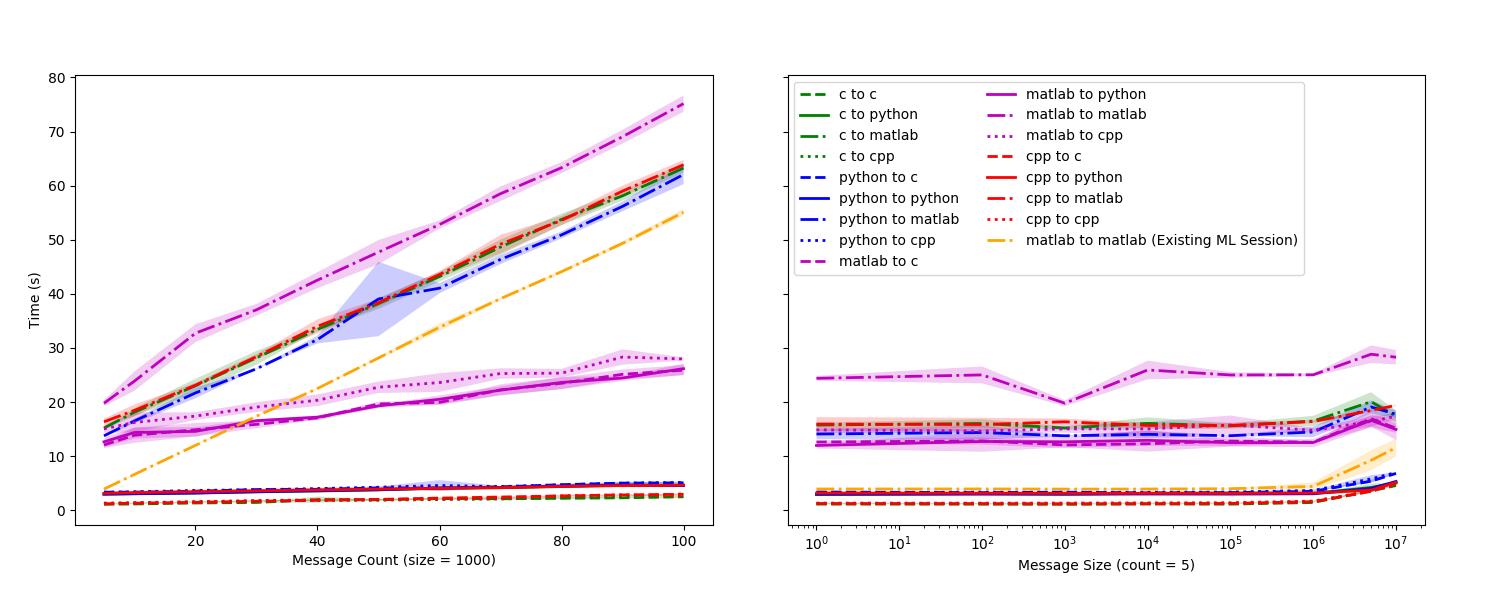
\includegraphics[width=\columnwidth,keepaspectratio]{./images/scaling_language_matlab.png}
	\caption{Comparison of communication time scaling between languages on Mac OS X including Matlab.}
	\label{fig:language_matlab}
	\end{center}
	\end{figure}
\fi
%
\begin{table}[htbp]
\begin{center}
\begin{tabular}{|c|c|c|c|}
\hline
Source 	& Destination 	& Time per Message (s) 	& Overhead (s) 	\\\hline
C 				& C					& 0.015				& 1.11			\\
C 				& C++				& 0.016				& 1.15			\\
C 				& Python				& 0.019				& 2.86			\\
C				& Matlab				& 0.505				& 12.98			\\
\hline%
C++ 				& C					& 0.019				& 1.10			\\
C++ 				& C++				& 0.016				& 1.25			\\
C++ 				& Python				& 0.016				& 3.10			\\
C++ 				& Matlab				& 0.505				& 13.45			\\
\hline%
Python			& C					& 0.019				& 3.17			\\
Python			& C++				& 0.019				& 3.26			\\
Python			& Python				& 0.019				& 2.86			\\
Python			& Matlab				& 0.500				& 11.61			\\
\hline%
Matlab			& C					& 0.144				& 11.82			\\
Matlab			& C++				& 0.142				& 14.79			\\
Matlab			& Python				& 0.139				& 12.23			\\
Matlab			& Matlab				& 0.559				& 19.28			\\
\hline%
Matlab (started)		& Matlab (started)		& 0.537				& 1.25			\\
\hline
\end{tabular}
\end{center}
\caption{Effect of model language on performance (Mac OS X) with Matlab.}
\label{tab:language_matlab}
\end{table}%
%

Except for Matlab models, the time required per message is not affected by the language of either model for smaller messages. There is a very small increase in the time per message when there is a Python model involved, but this is much lower than the standard deviation resulting from background activity on the test machine and so is in conclusive. Matlab models have a much higher time per message than any other language. This results from the way the Matlab interface was implemented, by calling the Python interface. The time required per message is largest when the receiving model is written in Matlab because the receiving models both receives messages from the other model and send output to a file, resulting in twice the number of calls to the wrapped interface. The performance of the Matlab interface may be improved in the future by either implementing it in Matlab directly or by wrapping the C routines.

Language also plays a role for messages larger than the maximum ($2^{20}$ bytes), when messages must be broken into smaller pieces. In particular, integrations that include a C or C++ receiving model scale more strongly than for those that have a Python receiving model because, in addition to the input/output connection drivers, the Python interface itself is asynchronous while the C/C++ interface is not. This means that while Python receiving models have concurrent operations to receive, backlog, and confirm messages, C/C++ models will block on each receive until the input connection driver completes the confirmation handshake. In addition, because C/C++ models are not continuously receiving and backlogging messages, the channel will become saturated. Once it reaches its maximum, the input connection driver can no longer pass along messages and must wait for the model to receive the next message. One remedy that is being explored for future releases, is to make the C/C++ interface asynchronous as well. However, this is a low priority as only models with very rapid and high volume input (such as the test models) are affected.

The largest difference between the different test cases is in in the overhead. Every model driver entails some overhead. For interpreted languages (e.g. Python and Matlab), the majority of the overhead comes from starting the interpreter. For Matlab, this is particularly time consuming ($>10$ s). Although this is only a one-time cost required at the start of an integration, {\cis} does offer ways to alleviate this if multiple runs are necessary by starting a Matlab engine prior to the first integration that can be used by subsequent runs. When Matlab is started in advance (the dashed-dotted orange line in Figure \ref{fig:language_matlab}), the overhead for Matlab models drops to 1.25\,s, less than Python (2.86\,s) but slightly more than C (1.11\,s).

For compiled languages (C and C++), the overhead comes from compiling the source code which is done in serial. The time required for compilation will depend on the compiler used and the complexity of the model code. For command line compiled models, {\cis} forces the model to be recompiled every time to ensure any changes to the source code are propagated. However, for models that use Make and CMake, overhead due to compile time can be reduced by using existing builds.

Interestingly, the recorded overheads were not symmetric or additive. For example, the Python-to-C integrations required more overhead than the C-to-Python integrations. This is because the models are started in parallel, but do not require the same amount of time to start and being execution. C models, while requiring compilation, start much faster than Python models. In a Python-to-C integration, the C model must wait for the Python model to finish its much slower startup and begin sending message, while in a C-to-Python integration, the C model can immediately begin sending messages that will be received by the Python model once it finishes starting up. In addition, the Python-to-Python integrations required less time than any of the other integrations that included Python because, although Python models take longer to start up, the start up is done in parallel while the compilation for the C and C++ models is done in serial. This source of overhead could be ameliorated by compiling models in parallel or in advanced, but is usually not significant enough to effect overall performance.


% PYTHON VERSION
\subsection{Python Version}\label{SS:results_python}
%
Figure \ref{fig:python} and Table \ref{tab:python} compare the execution times when using different versions of Python. The performance tests for both Python 2.7 and Python 3.5 were performed on the Linux machine from above using ZeroMQ communication and two different integration (Python-to-Python and C-to-C).
%
\ifinclfig
 	\begin{figure}[htbp]
	\begin{center}
	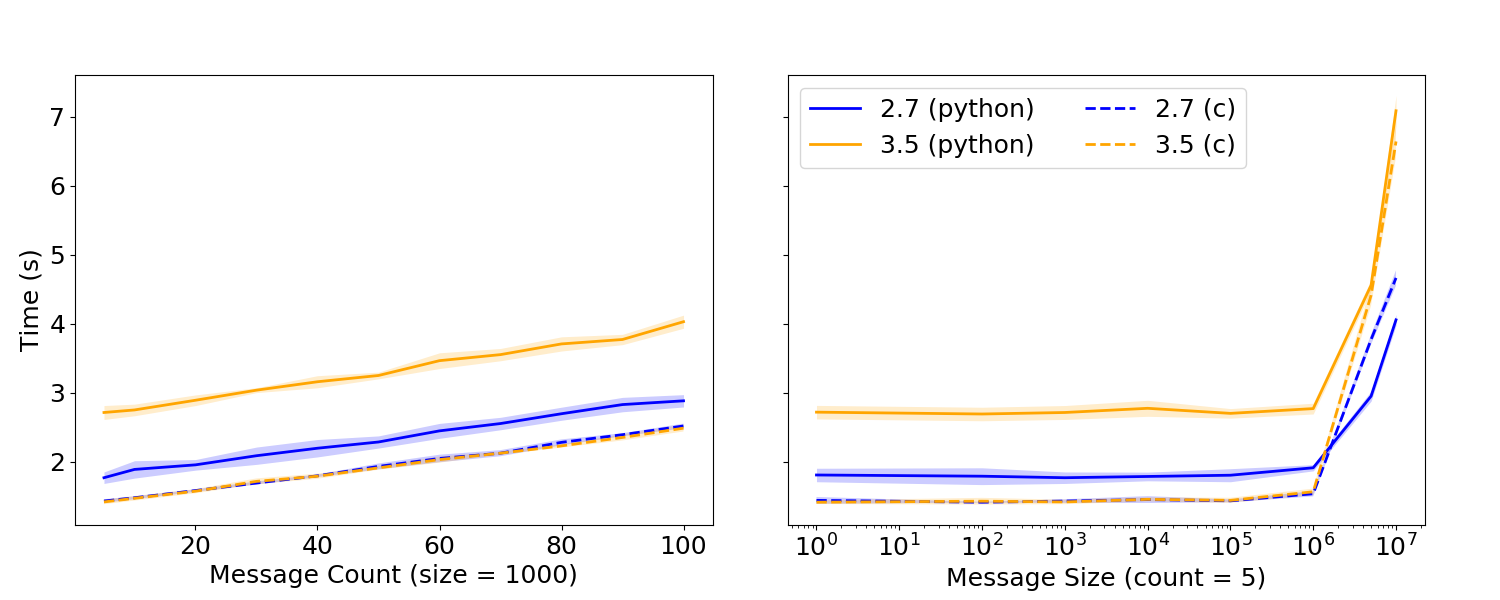
\includegraphics[width=\columnwidth,keepaspectratio]{./images/scaling_python.png}
	\caption{Comparison of communication time scaling between Python versions on Linux. The solid lines are for the Python-to-Python integrations and the dotted lines are for the C-to-C integration.}
	\label{fig:python}
	\end{center}
	\end{figure}
\fi
%
\begin{table}[htbp]
\begin{center}
\begin{tabular}{|c|c|c|c|}
\hline
Python Version	& Language	& Time per Message (s) 	& Overhead (s) 	\\\hline
2.7			& Python		& 0.012				& 1.73			\\
2.7			& C			& 0.011				& 1.36			\\
3.5 			& Python		& 0.013				& 2.62			\\
3.5			& C			& 0.011				& 1.36			\\\hline
\end{tabular}
\end{center}
\caption{Effect of Python version on performance.}
\label{tab:python}
\end{table}          
%
There is $\sim1$\,s additional overhead with Python 3.5 compared to Python 2.7 due to the increased startup time for the Python 3.5 interpreter. This overhead is only present for integrations that include Python models. For comparison, there is no difference in the time per message and overhead between the different Python versions for the C-to-C integration (dashed lines in Figure \ref{fig:python}). There is a slight difference in time per message between the two versions for all models that shows up in the scaling of execution time with message size for large messages ($>10^6$ bytes). Differences at large message sizes between the two versions arrises from the use of Python drivers to transport messages between models and is more pronounced in integrations with Python models due to the increased amount of Python code.

% PLATFORM
\subsection{Operating System}\label{SS:results_platform}
%
Figure \ref{fig:platform} and Table \ref{tab:platform} compare the execution times on different operating systems. The performance tests reported for Linux were run on the machine from above. The tests for Mac OS X were run on a 2015 MacBook Pro with a 2.9 GHz Intel Core i5 processor running macOS High Sierra 10.13.4. The tests for Windows were run on the same machine from a dual boot of Windows 10. All platform dependent performance tests use ZeroMQ communication and the Python-to-Python integration.
%
\ifinclfig
 	\begin{figure}[htbp]
	\begin{center}
	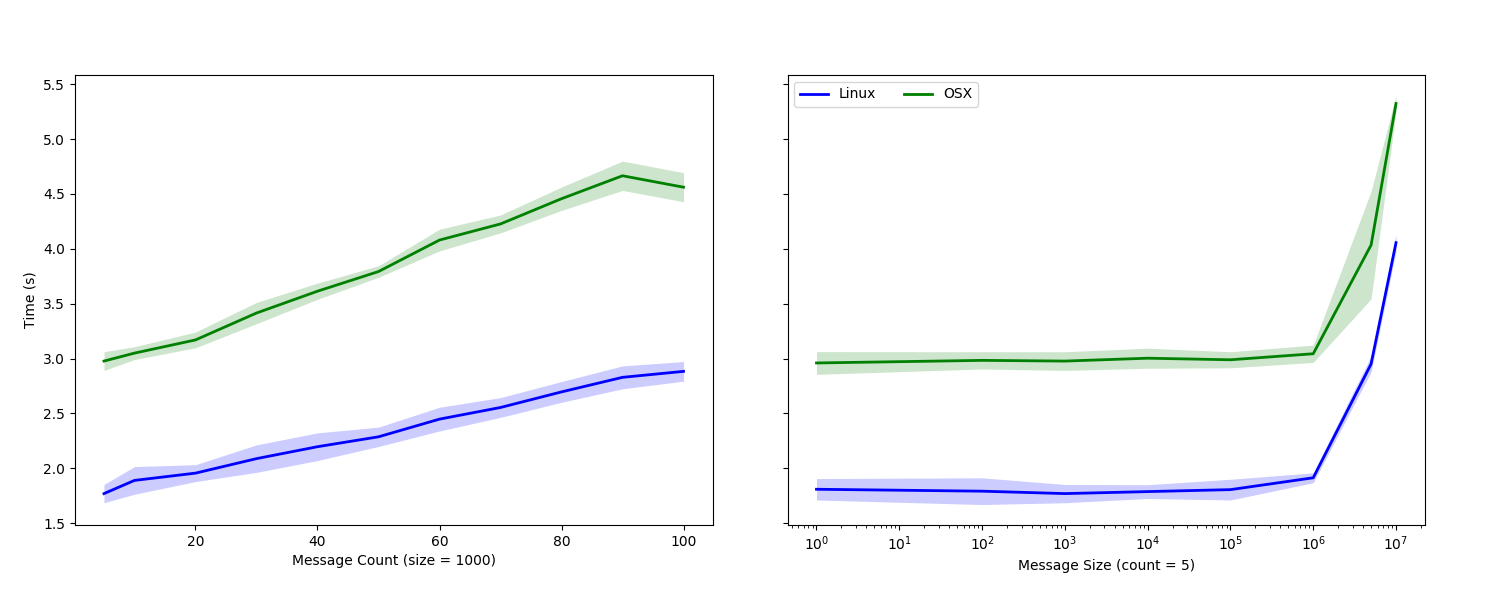
\includegraphics[width=\columnwidth,keepaspectratio]{./images/scaling_platform.png}
	\caption{Comparison of communication time scaling between operating systems.}
	\label{fig:platform}
	\end{center}
	\end{figure}
\fi
%
\begin{table}[htbp]
\begin{center}
\begin{tabular}{|c|c|c|}
\hline
Operating System	& Time per Message (s) 	& Overhead (s) 	\\\hline
Linux			& \todo{?}				& \todo{?}			\\
Mac OS X			& \todo{?}				& \todo{?}			\\
Windows			& \todo{?}				& \todo{?}			\\\hline
\end{tabular}
\end{center}
\caption{Effect of operating system on performance.}
\label{tab:platform}
\end{table}%
%
\todo{Windows results \& discussion}

%---------------------------------------------------------------------------------
%---------------------------------------------------------------------------------
% SUMMARY & DISCUSSION
\section{Summary \& Discussion}\label{S:discuss}

%---------------------------------------------------------------------------------
% CURRENT STATUS
\subsection{Current Status}\label{SS:current}
%
{\cis} is an open-source Python package for connecting computational models across programming languages and scales to form integration networks. Models are run in parallel with asynchronous message passing handled under-the-hood via threading and one of three communication mechanisms. {\cis} works on Linux, Mac OS X, and Windows operating systems with Python 2.7, 3.4, 3.5, 3.6 and 3.7. {\cis} currently supports running models written in Python, C, C++, and Matlab with additional support for compiling models C/C++ using Make \citep{Stallman2004} or CMake \citep{Martin2006} and running models written in the LPy \citep{Boudon2012} DSL.

{\cis} has already been used to integrate several plant models within the Crops in Silico organization with ongoing work to add additional models to the integration network. Figure \ref{fig:network} shows the progress so far. Each square is a model and lines between the models represent connections where information is exchanged. Solid lines are connections that have already implemented, dashed lines are connections currently being implemented, and dotted lines are connections planned for the future. Results from one integration, a metabolic model and genetic response to CO$_2$ model, can be found in 
%
\ifieee
	\citep{integration_prep}. 
\else
	\citet{integration_prep}. 
\fi
%
\ifinclfig
 	\begin{figure}[htbp]
	\begin{center}
	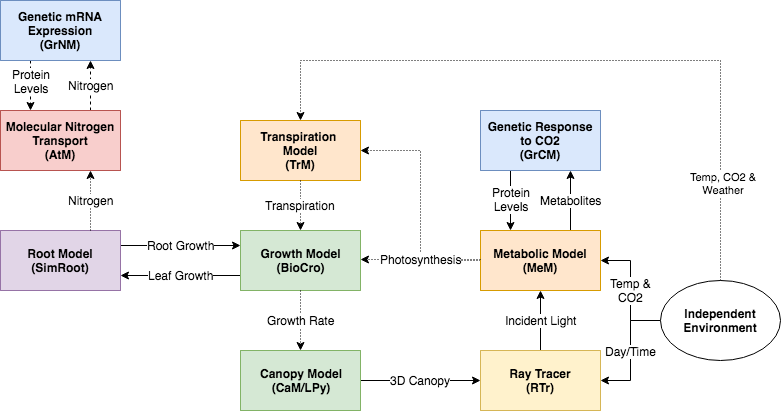
\includegraphics[width=\columnwidth,keepaspectratio]{./images/CiS-BioCro-Planned.png}
	\caption{Progress towards full Crops in Silico integration network.}
	\label{fig:network}
	\end{center}
	\end{figure}
\fi
%
\todo{more here? teaser results?}

%---------------------------------------------------------------------------------
% FUTURE WORK
\subsection{Current/Future Improvements}\label{SS:future}
%
{\cis} is being actively developed to expand the number of models 
that can be used in integration networks and the complexity of integration 
networks that can be executed. Several improvements are already in progress/planned for {\cis}.

% LANGUAGE SUPPORT
\subsubsection{Language Support}\label{SS:langsupport}
%
The biggest barrier to running new models is language support. Plant models 
are written in many different languages. While the current language support 
covers many of the most popular languages among plant biologists, 
additional languages must be added to unlock the full set of potential integrations. 
Surveys of the plant modeling community have helped identify the core languages 
that models have been written in. Based on these results, we plan to expand 
{\cis} to support models written in R, Fortran, Java, and the SBML \citep{Hucka2003} DSL.

We also plan to add support for running Matlab models using Octave \citep{Eaton2002}. Matlab 
models require a Matlab license to run. Given that plant modelers do not all 
use Matlab, it cannot be assumed that everyone will have access to a Matlab 
license. Octave is open source and provides much of the same functionality 
as Matlab and can run many Matlab codes. Support for Octave will improve 
modelers ability to collaborate without worrying about access to a Matlab 
license. 

% DISTRIBUTED SYSTEMS
\subsubsection{Distributed Systems}\label{SS:distributed}
%
High performance computing (HPC) and cloud compute resources are powerful 
tools in the current computing ecosystem that could be used for running 
complex integration networks. To this end, we plan to expand {\cis} 
support for running integration networks on distributed compute resources. 
{\cis} already uses communication tools that can be adapted for use 
in a distributed pattern. We will leverage tools like the libsubmit package from the 
Parsl project \citep{babuji18} for 
automating the submission process to HPC and compute resources. In addition, 
we will add tools for running models as a service and using RabbitMQ to 
permit access to these models within integration networks.

% CONTROL FLOW
\subsubsection{Control Flow}\label{SS:control}
%
Currently, modelers must explicitly specify how a model should process input 
within the model code including things like which input variables are static 
and received once versus which variables change and should be looped over. 
We plan on adding options to {\cis} for dynamically generating model code 
based a user provided function call and list of static/variable input channels. 
This will allow better reusability of model code such as during parameter studies.

% DATA AGGREGATIOIN
\subsubsection{Data Aggregation}\label{SS:dataagg}
%
Much of the original version of {\cis} centered around the use of 
tabular input data. While tabular data is used heavily by plant models, it 
presents several barriers for constructing integration networks. Tabular input 
data only works when one model outputs the same columns that are expected as 
input by another model. However, this is unlikely to be the case if two models 
are developed independently. Future improvements to {\cis} will allow 
tabular input to models to be composed by aggregating output data from more than 
one model and/or file.

% JSON DATA TYPE SPECIFICATION
\subsubsection{JSON Data Type Specification}\label{SS:json}
%
While {\cis} supports serialization of several data types/formats, we 
would like to make serialization as flexible as possible. To this end, 
{\cis} will be adapted to read JSON schema \citep{jsonschema} for user defined types that 
can be used to automatically create the appropriate data structures alongside
methods for parsing and serializing them.

% GUI
\subsubsection{Graphical User Interface}\label{SS:gui}
%
In an effort to make {\cis} as user friendly as possible, we have also begun work on a graphical user interface (GUI) for entering model information, composing integration networks from an existing palette of models, and displaying basic output from an integration run. The current prototype of the GUI can only handle model ingestion and network composition; model execution must be done locally. However, our ultimate goal with the GUI is to provide a service where users can register their model, compose and run integration networks on dedicated cloud compute resources, and view output in real time all from the web browser. 
%\todo{Provide \href{https://hackathon.cis.ndslabs.org/}{link?}}

%---------------------------------------------------------------------------------
% CODE
\section*{Code}\label{S:code}
The {\cis} package is available publicly on \href{https://github.com/cropsinsilico/cis_interface}{Github} and can be 
installed using {\tt pip} or {\tt conda}. To ensure code health, {\cis} boasts 100\% code coverage with automated testing on Linux, Mac OS X, and Windows for Python version 2.7, 3.4, 3.5, 3.6, and 3.7 via continuous integration with TravisCI \citep{travisci} and Appveyor \citep{appveyor}. Full documentation for {\cis} can be found \href{https://cropsinsilico.github.io/cis_interface/}{here} including step-by-step directions from the tutorial conducted during the \href{https://cropsinsilico.github.io/cis_interface/hackathon2018/index.html}{2018 Crops in Silico Hackathon}.

%---------------------------------------------------------------------------------
% TODO
\todo{%
\section*{TODO}
\begin{itemize}
	\item Fix code citations to include URLs
	\item Increase size of font on figures or increase size of figures (depends on iSP format)
	\item Get real in-prep citation from Kavya
	\item Confirm sentence about Yu/Kavya integration for accuracy
	\item Get grant numbers/titles for acknowledgments
	\item Ask Matt about author list
	\item Add plots that include Windows results when they finish
	\item Include statistics in tables on scaling at large message size?
	\item Re-run Matlab-to-Matlab, $nmsg=5$, $msg\_size=1000$
\end{itemize}
}

%---------------------------------------------------------------------------------
% ACKNOWLEDGMENTS
\section*{Acknowledgments}
\ifieee
\else
\acknowledgments
\fi
%
This work was supported by funding from the Foundation for Food and Agriculture Research (FFAR), Institute for Sustainability, Energy, and Environment (iSEE), and the National Center for Supercomputing Applications (NCSA).
The authors would like to thank Mike Lambert and Craig Willis for their ongoing work on a graphical user interface for visually composing and running integration networks for {\cis} as well as David Raila for his work on the original integration code that {\cis} was based on.

%---------------------------------------------------------------------------------
% REFERENCES
\ifdraft
	\bibliography{CiS}
\else
	\input{ms-bbl.tex}
\fi

%---------------------------------------------------------------------------------
% FIGURES
\ifplacefig
\else
% put figures here if figures go after
\fi

%---------------------------------------------------------------------------------
% COMMENTS
%\newpage
%\todo{To do:
%\begin{itemize}
%\item Improve conclusion
%\item Non-uniform test data set?
%\item Performance of runs on cosmology dataset?
%\item Move figures to the end for submission
%\item iPython notebook for running tests
%\end{itemize}
% }

\end{document}
